\documentclass{article}
\usepackage{amsmath}
\usepackage{amsfonts}
\usepackage{bm}
\usepackage[theorems]{mymacros}
\usepackage{graphicx}
\usepackage{paralist}
\usepackage{comment}
\usepackage{url}
\usepackage{tikz}
\usepackage{smallref}
\usepackage{enumitem}
\usetikzlibrary{arrows}
\usepackage[margin=1in]{geometry}
\newcommand\ddadbdc[3]{\frac{\partial^2 #1}{\partial #2 \partial #3}}
\newcommand\rowvector[1]{\left( \begin{array}{c} #1 \end{array} \right)}
\newcommand\de[1]{\mathrm{de}({#1})}
\newcommand\at{\Bigg|}
\newcommand\question[1]{\noindent \textit{#1}}
\newcommand\alert[1]{\textbf{#1}}
\newcommand{\ot}{\leftarrow}
\newcommand{\oto}{\leftrightarrow}
\newcommand{\ots}{\leftarrow\mkern-13mu\ast\,}
\newcommand{\sto}{\,\ast\mkern-13mu\to}
\newcommand{\stt}{\,\ast\mkern-13mu\relbar\!\!\!\relbar}
\newcommand{\tts}{\relbar\!\!\!\relbar\mkern-13mu\ast\,}
\DeclareMathOperator{\intervene}{do}
%\setlength\parskip{0.5\baselineskip}
%\setlength\parindent{0pt}
\tikzstyle{var}=[circle,draw,fill=white,thick,minimum size=20pt,inner sep=0pt]
\tikzstyle{varh}=[circle,draw,fill=gray!10,thick,minimum size=20pt,inner sep=0pt,dotted]
\tikzstyle{arr}=[->,>=stealth',draw,thick]
%\tikzstyle{arr}=[->,>=stealth',draw=black,fill=black,line width=1pt]
%\tikzstyle{arrh}=[->,>=stealth',draw=gray,thin]
\tikzstyle{arrh}=[->,>=stealth',draw,fill=gray,thick,dotted]
\tikzstyle{biarr}=[<->,>=stealth',draw,fill=black,thick]
\tikzstyle{fac}=[rectangle,draw=black!50,fill=black!20,thick,minimum size=10pt] %or 15pt
\tikzstyle{vari}=[circle,draw=white,fill=red,thick,minimum size=20pt,inner sep=0pt]
\title{Exercises MLSS 2019: \emph{Causality}}
\author{Joris Mooij}
\date{August 27, 2019}
\begin{document}
\maketitle
\section{In-class exercises}
\subsection{Simpson's Paradox}
%\nocite{Pearl99}
You are investigating the effectiveness of a drug against a deadly disease.
You are given access to data collected by health insurance companies about
their customers. You divide the diseased customers into two groups: those 
that took the drug, and those that didn't take the drug. 
Some of the customers
recovered, others unfortunately didn't recover. The reasons why some patients
were treated and others were not, are unknown to you. 
You find the following numbers:\\

\centerline{\begin{tabular}{l|cc|c|c}
 & Recovery & No recovery & Total & Recovery rate \\
\hline
Drug    & 20 & 20 & 40 & \dots\% \\
No drug & 16 & 24 & 40 & \dots\% \\
\hline
Total   & 36 & 44 & 80 & \\
\end{tabular}}

\begin{enumerate}[label=\alph*)]
\item \question{Calculate the recovery rates (in \%) for both groups (``drug'' and ``no drug'').}
  \answer{Drug: 50\%; No drug: 40\%.}

\item \question{If you were diseased, would you take the drug, or not?}
\answer{The data provided does not contain enough information to decide rationally (at first sight, one might think that taking the drug is advantageous).}
\end{enumerate}

Upon closer inspection of the data, you notice something peculiar when you group patients according to gender:\\

\centerline{\begin{tabular}{l|cc|c|c}
\textbf{Males} & Recovery & No recovery & Total & Recovery rate \\
\hline
Drug    & 18 & 12 & 30 & \dots\% \\
No drug &  7 &  3 & 10 & \dots\% \\
\hline
Total   & 25 & 15 & 40 & \\
\end{tabular}}
\medskip
\centerline{\begin{tabular}{l|cc|c|c}
\textbf{Females} & Recovery & No recovery & Total & Recovery rate \\
\hline
Drug    &  2 &  8 & 10 & \dots\% \\
No drug &  9 & 21 & 30 & \dots\% \\
\hline
Total   & 11 & 29 & 40 & \\
\end{tabular}}

\begin{enumerate}[resume*]
  \item \question{Calculate the recovery rates (in \%) for both groups (``drug'' and ``no drug''), for each subpopulation (males and females) separately.}
\answer{Males: Drug 60\%; No drug 70\%.\\
Females: Drug 20\%; No drug 30\%.}

  \item \question{In light of these numbers, would you take the drug if you were diseased, or not?}
\answer{The data provided does not contain enough information to decide rationally (at first sight, one might think that taking the drug is disadvantageous for both males and females).}

  \item \question{What would be your advice to a diseased patient with unknown gender?}
\answer{The data provided does not contain enough information to decide rationally.}
\end{enumerate}

This phenomenon is known as ``Simpson's paradox''.
A lot has been written about this paradox, but it dissolves once you recognize that you should not make the mistake of interpreting correlations as causations, as we'll see later today.

%\bibliographystyle{apalike}
%\bibliography{lecture}

\subsection{Paths, colliders, d-blocked paths and d-separation}

  \begin{definition}[Paths, Ancestors]
  Let $\C{G}$ be a directed mixed graph.
    \begin{compactitem}
      \item A \alert{path} $q$ in $\C{G}$ is a sequence of adjacent edges in $\C{G}$ in which no node occurs more than once.
      \item A path consisting of directed edges $X_{i_1} \to X_{i_2} \to X_{i_3} \to \dots \to X_{i_k}$ that all point in the same direction is called a \alert{directed} path.
      \item If there is a directed path from $X$ to $Y$ (or if $X=Y$), $X$ is called an \alert{ancestor} of $Y$.
      \item The ancestors of $Y$ are denoted \alert{$\an_{\C{G}}(Y)$}, and include $Y$.
      \item For a set of nodes $\B{Z}$, $\an_{\C{G}}(\B{Z}) := \bigcup_{Y \in \B{Z}} \an_{\C{G}}(Y)$.
    \end{compactitem}
  \end{definition}
  \begin{definition}[Colliders, Blocked Paths, $d$-separation]
    Let $\C{G}$ be a directed mixed graph, and $q$ a path on $\C{G}$.
    \begin{compactitem}
      \item A \alert{collider} on $q$ is a (non-endpoint) node $X$ on $q$ with precisely two arrowheads pointing towards $X$ on the adjacent edges:\hfil
    $$\rightarrow X \leftarrow, \quad \rightarrow X \leftrightarrow, \quad \leftrightarrow X \leftarrow, \quad \leftrightarrow X \leftrightarrow$$
     \item A \alert{non-collider} on $q$ is any node on the path which is not a collider.
    \end{compactitem}

    A set of nodes $\B{S}$ in $\C{G}$ is said to \alert{d-block} $q$ if $q$ contains
    a non-collider which is in $\B{S}$, or a collider which is \emph{not} an ancestor of $\B{S}$.

    For three sets $\B{X},\B{Y},\B{Z}$ of nodes in $\C{G}$, we say that
    \alert{$\B{X}$ and $\B{Y}$ are $d$-separated by $\B{Z}$} iff all paths between a node in $\B{X}$ and a node in $\B{Y}$ are d-blocked by $\B{Z}$, and write \alert{$\B{X} \dsep_{\C{G}} \B{Y} \given \B{Z}$}.
  \end{definition}
    
%  \clearpage
  \noindent Consider the following directed mixed graph $\C{G}$:\\

  \centerline{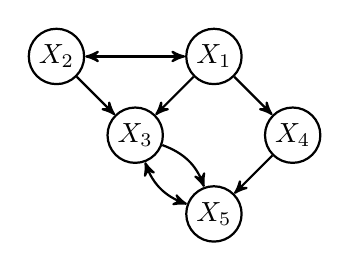
\begin{tikzpicture}
      \node[var] (X1) at (5,-0.5) {$X_1$};
      \node[var] (X2) at (3,-0.5) {$X_2$};
      \node[var] (X3) at (4,-1.5) {$X_3$};
      \node[var] (X4) at (6,-1.5) {$X_4$};
      \node[var] (X5) at (5,-2.5) {$X_5$};
      \draw[arr] (X1) edge (X3);
      \draw[arr] (X1) edge (X4);
      \draw[arr] (X2) edge (X3);
      \draw[arr] (X4) edge (X5);
      \draw[biarr] (X1) edge (X2);
      \draw[arr,bend left=25] (X3) edge (X5);
      \draw[biarr,bend right=25] (X3) edge (X5);
  \end{tikzpicture}}
    
  \begin{enumerate}[label=\alph*)]
  \item \question{Is $X_3 \rightarrow X_5 \leftrightarrow X_3$ a path? Is it a directed path?}
  \answer{It is neither, as the node $X_3$ appears more than once.}

  \item \question{Is $X_3 \leftrightarrow X_5$ a path? Is it a directed path?}
  \answer{It is a path (a single edge counts as a sequence of edges) but it is not directed, as it contains a bidirected edge.}

  \item \question{Is $X_5 \leftarrow X_3 \leftarrow X_1$ a path? Is it a directed path?}
  \answer{Yes, it is a path, and it is a directed path (from $X_1$ to $X_5$).}

  \item \question{What are the ancestors of $X_4$?}
  \answer{$\an_\C{G}(X_4) = \{X_1,X_4\}$.}
  \end{enumerate}
 
  Consider the path $X_2 \leftrightarrow X_1 \rightarrow X_3 \leftrightarrow X_5 \leftarrow X_4$ on $\C{G}$. 

  \begin{enumerate}[resume*]
    \item \question{Which nodes on the path are colliders?}
  \answer{$X_3$ and $X_5$ are colliders on this path.}

  \item \question{Which nodes on the path are non-colliders?}
  \answer{$X_2$, $X_1$, $X_4$ are non-colliders on this path.}
%  \question{2c. Which subsets of $\{X_1,X_3,X_5\}$ block this path?}\\
%  \answer{$\emptyset, \{X_1\}, \{X_3\}, \{X_1,X_3\}, \{X_5\}, \{X_1,X_5\}, \{X_1,X_3,X_5\}$.\\}
%  \question{2d. Which subsets of $\{X_1,X_3,X_5\}$ d-separate $X_2$ from $X_4$?}\\
%  \answer{}
  \item \question{Does $\{X_3\}$ d-block this path? Does $\{X_5\}$ d-block this path? Does $\{X_3,X_5\}$ d-block this path?}
  \answer{Yes, Yes, No.}

  \item \question{Does $X_1$ d-separate $X_2$ from $X_4$?}
  \answer{Yes.}

  \item \question{Is $X_1 \dsep X_5 \given \{X_3,X_4\}$?}
  \answer{No: the path $X_1 \to X_3 \oto X_5$ is not d-blocked by $\{X_3,X_4\}$.}
  \end{enumerate}

\clearpage
\section{Tutorial exercises}

\subsection{Seeing vs.\ Doing in SCMs}

Consider a simple causal model of a car. The endogenous variables are (all binary):
\begin{center}
\begin{tabular}{ll}
    $X$: the battery is charged \\
    $Y$: the start engine is operational \\
    $S$: the car starts
\end{tabular}\end{center}
The exogenous variables (latent, independent, binary) have Bernoulli distributions:
  \begin{align*}
    E_X &\sim \mathrm{Ber}(0.95) \\
    E_Y &\sim \mathrm{Ber}(0.99) \\
    E_Z &\sim \mathrm{Ber}(0.999)
  \end{align*}
The structural equations are specified by:
  \begin{align*}
    X &= E_X \\
    Y &= E_Y \\
    S &= X \land Y \land E_S
  \end{align*}
where ``$\land$'' is the logical AND.

\begin{enumerate}[label=\alph*)]
  \item \question{Draw the corresponding augmented causal graph and the causal graph.}
\answer{
  
  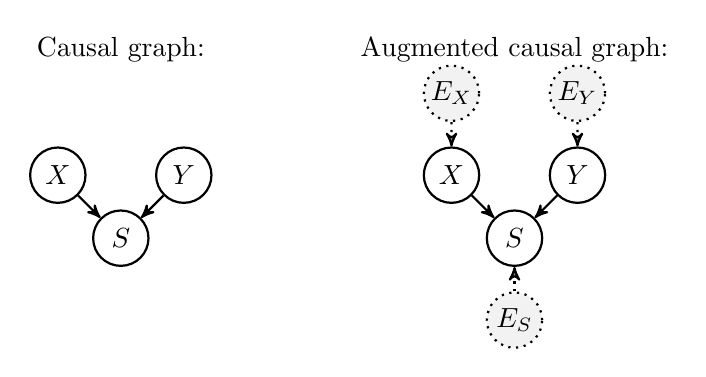
\begin{tikzpicture}
    \begin{scope}[scale=0.8]
      \node at (0,3) {Causal graph:};
      \node[var] (X1) at (-1,1) {$X$};
      \node[var] (X2) at (1,1) {$Y$};
      \node[var] (X3) at (0,0) {$S$};
      %\only<1-2>{
        \draw[arr] (X1) edge (X3);
        \draw[arr] (X2) edge (X3);
      %}
    \end{scope}
    \begin{scope}[xshift=5cm,scale=0.8]
      \node at (0,3) {Augmented causal graph:};
      \node[varh] (E1) at (-1,2.3) {$E_X$};
      \node[varh] (E2) at (1,2.3) {$E_Y$};
      \node[varh] (E3) at (0,-1.3) {$E_S$};
      \node[var] (X1) at (-1,1) {$X$};
      \node[var] (X2) at (1,1) {$Y$};
      \node[var] (X3) at (0,0) {$S$};
      %\only<1,3>{
      \draw[arrh] (E1) edge (X1);
      %}
      \draw[arrh] (E2) edge (X2);
%      \only<1-2>{
        \draw[arrh] (E3) edge (X3);
        \draw[arr] (X1) edge (X3);
        \draw[arr] (X2) edge (X3);
%      }
    \end{scope}
\end{tikzpicture}}

\item \question{Write pseudocode to draw a sample $(x,y,s)$ from this model.}
\answer{Draw $x \sim \mathrm{Ber}(0.95)$. Draw $y \sim \mathrm{Ber}(0.99)$. Draw $e_S \sim \mathrm{Ber}(0.999)$. Calculate $s := x \land y \land e_S$.}

\item \question{How does the model change under a perfect intervention $\intervene(S=0)$? Write down the intervened model. How does the pseudocode to sample from the model change?}
\answer{The exogenous distribution remains the same. The intervened structural equations are:
  \begin{align*}
    X &= E_X \\
    Y &= E_Y \\
    S &= 0.
  \end{align*}
The change to the sampler is the last step, which is replaced by $s := 0$.
}

%\item \question{Is $p(X=x|S=s) = p(X=x|\intervene(S=s))$? Motivate your answer.}
%\answer{No: observing $S$ provides information about the value of $X$ (e.g., observing that the car doesn't start makes it more likely that the battery is empty). Since $S$ is not a cause of $X$, intervening on $S$ does not lead to a change of the value of $X$.}

%\item \question{Is $p(S=s|X=x) = p(S=s|\intervene(X=x))$? Motivate your answer.}
%\answer{Yes: $S$ is a direct effect of $X$, and the two do not have an observed or unobserved confounder, hence seeing is the same as doing in this case.}

\item \question{Calculate:
  \begin{enumerate}[label=\roman*)]
  \item $p(S=1)$ (the probability that the car starts)
  \item $p(S=1|X=1)$ (the probability that the car starts, given that the battery is charged)
  \item $p(S=1|\intervene(X=1))$ (the probability that the car starts when we charge the battery)
\end{enumerate}}
\answer{\begin{enumerate}[label=\roman*)]
  \item $p(S=1) = \sum_{x=0}^1 \sum_{y=0}^1 p(S=1,X=x,Y=y) = 0.95 \times 0.99 \times 0.999 \approx 0.934$
  \item $p(S=1|X=1) = \sum_{y=0}^1 p(S=1|X=1,Y=y) p(Y=y) = 0.999 \times 0.99 \approx 0.989$
  \item $p(S=1|\intervene(X=1)) = \sum_{y=0}^1 p(S=1|X=1,Y=y) p(Y=y) = 0.999 \times 0.99 \approx 0.989$
\end{enumerate}}

\item \question{Calculate:
\begin{enumerate}[label=\roman*)]
  \item $p(X=0)$ (the probability that the battery is empty)
  \item $p(X=0|S=0)$ (the probability that the battery is empty given that the car fails to start)
  \item $p(X=0|\intervene(S=0))$ (the probability that the battery is empty if we lost the key)
\end{enumerate}}
\answer{\begin{enumerate}[label=\roman*)]
  \item $p(X=0) = 0.05$
  \item \begin{equation*}\begin{split}
    p(X=0|S=0) 
    &= \frac{p(S=0,X=0)}{p(S=0)} \\
    &= \frac{p(S=0|X=0)p(X=0)}{\sum_{x=0}^1 \sum_{y=0}^1 p(X=x,Y=y,S=0)} \\
    &= \frac{1 \times 0.05}{0.05 \times 0.01 + 0.95 \times 0.01 + 0.05 \times 0.99 + 0.95 \times 0.99 \times 0.001} \\
    &\approx 0.827
  \end{split}\end{equation*}
  \item $p(X=0|\intervene(S=0)) = 0.05$
\end{enumerate}}

\end{enumerate}

%\begin{itemize}
%  \item Calculate $p(X,Y)$
%  \item Is $X \indep Y$?
%\end{itemize}
%A car mechanic only observes cars that don't start. Calculate:
%\begin{itemize}
%  \item Calculate $p(X,Y|S=1)$ and $p(X,Y|S=0)$.
%  \item Is $X \indep Y \given S$?
%  \item What does Reichenbach's Principle of Common Cause tell you about $X$ and $Y$?
%\end{itemize}

\subsection{The Back-Door Criterion}

\begin{comment}
Question: does the original formulation below still work in the cyclic case?
No directed path $X \to \dots \to H$ implies no directed path $I_X \to \dots \to H$
which covers part of $H \indep I_X$. If we start from $I_X$ with a directed path
and encounter a collider along the way before arriving at $H$ then that path will
also be d-blocked. So yes, $H \indep I_X$ is guaranteed. Second,
$Y \indep I_X \given X, H$. Consider the paths $I_X \to X \dots Y$. If the part
between $X$ and $Y$ is a back-door path, i.e., it starts as $I_X \to X \ots \dots Y$
it is d-blocked by $H$. Is it then
$\sigma$-blocked? If it isn't a back-door path, it starts as $I_X \to X \to Z$. 
This is $\sigma$-blocked by $X$ except if $Z$ is in the scc of $X$. 

Counterexample: $I_X \to X \to Y \to Z \to X$. Here, we don't have
$Y \indep I_X \given X,Z$ even though it satisfies the formulation below.
Ah no, now $Z$ is ancestor of $X$.

So in addition let us assume that $Y$ is not ancestor of $X$. 

$I_X \to X \ot H \ot Y$ so $p(Y) = p(Y|\intervene(X)) = \int p(Y|X,H) p(H) dH = \int p(Y|H) p(H) dH = p(Y)$

\begin{theorem}[Back-Door Criterion (Pearl, 2000)]
  For an acyclic SCM $\C{M}$, variables $X$, $Y$ and set of variables $\B{H}$: if
  \begin{compactenum}
  \item $X, Y \notin \B{H}$;
  \item $X$ is not an ancestor of any variable in $\B{H}$ in $\C{G}(\C{M})$;
  \item $\B{H}$ blocks all \alert{back-door paths} $X \leftarrow \dots Y$ and $X \leftrightarrow \dots Y$ in $\C{G}(\C{M})$ (i.e., all paths between $X$ and $Y$ that start with an arrowhead at $X$).
  \end{compactenum}
  then $\B{H}$ is called \emph{admissible for adjustment} to find the causal effect of $X$ on $Y$, and this causal effect is given by:
    $$p_{\C{M}}\big(y \given \intervene(X=x)\big) = \int p_{\C{M}}(y \given x, \B{h}) p_{\C{M}}(\B{h}) \,d\B{h} \left( {} = \sum_{\B{h}} p_{\C{M}}(y \given x, \B{h}) p_{\C{M}}(\B{h})\right).$$
  For the special case $\B{H} = \emptyset$, this should be read as:
  $$p_{\C{M}}\big(y \given \intervene(X=x)\big) = p_{\C{M}}(y \given x).$$
\end{theorem}
\end{comment}

\begin{theorem}[Back-Door Criterion (Pearl, 2000)]
  For an acyclic SCM $\C{M}$, variables $X$, $Y$ and set of variables $\B{H}$: 
  Let $\hat{\C{G}}$ be $\C{G}(\C{M})$ extended with an intervention node $I_X \to X$. If
  \begin{compactenum}
  \item $X, Y \notin \B{H}$;
  \item $\B{H} \dsep_{\hat{\C{G}}} I_X \given \emptyset$;
  \item $Y \dsep_{\hat{\C{G}}} I_X \given \{X\} \cup \B{H}$,
  \end{compactenum}
  then $\B{H}$ is called \emph{admissible for adjustment} to find the causal effect of $X$ on $Y$, and this causal effect is given by:
    $$p_{\C{M}}\big(y \given \intervene(X=x)\big) = \int p_{\C{M}}(y \given x, \B{h}) p_{\C{M}}(\B{h}) \,d\B{h} \left( {} = \sum_{\B{h}} p_{\C{M}}(y \given x, \B{h}) p_{\C{M}}(\B{h})\right).$$
  where the last equation only applies if $\B{H}$ is discrete-valued.
  For the special case $\B{H} = \emptyset$, this should be read as:
  $$p_{\C{M}}\big(y \given \intervene(X=x)\big) = p_{\C{M}}(y \given x).$$
\end{theorem}

  Consider an SCM $\C{M}$ with the following causal graph $\C{G}(\C{M})$:\\
  \begin{center}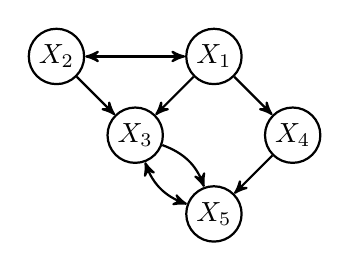
\begin{tikzpicture}
    \node[var] (X1) at (5,-0.5) {$X_1$};
    \node[var] (X2) at (3,-0.5) {$X_2$};
    \node[var] (X3) at (4,-1.5) {$X_3$};
    \node[var] (X4) at (6,-1.5) {$X_4$};
    \node[var] (X5) at (5,-2.5) {$X_5$};
    \draw[arr] (X1) edge (X3);
    \draw[arr] (X1) edge (X4);
    \draw[arr] (X2) edge (X3);
    \draw[arr,bend left=25] (X3) edge (X5);
    \draw[arr] (X4) edge (X5);
    \draw[biarr] (X1) edge (X2);
    \draw[biarr,bend left=25] (X5) edge (X3);
  \end{tikzpicture}\end{center}

  \begin{enumerate}[label=\alph*)]
    \item   \question{Give a set that is admissible for adjustment to find the causal effect of $X_4$ on $X_5$.}
  \answer{It must contain $X_1$ (so $\{X_1\}$, $\{X_1,X_2\}$, $\{X_1,X_3\}$, $\{X_1,X_2,X_3\}$).}

\item   \question{Provide an expression for this causal effect in terms of the observational distribution.}
  \answer{$$p_{\C{M}}\big(x_5 \given \intervene(X_4=x_4)\big) = \int p_{\C{M}}(x_5 \given x_4, x_1) p_{\C{M}}(x_1) \,dx_1.$$}

\item   \question{Give a set that is admissible for adjustment to find the causal effect of $X_1$ on $X_5$.}
  \answer{The only set that satisfies the sufficient condition of the back-door criterion is $\{X_2\}$.}

\item   \question{Provide an expression for this causal effect in terms of the observational distribution.}
  \answer{$$p_{\C{M}}\big(x_5 \given \intervene(X_1=x_1)\big) = \int p_{\C{M}}(x_5 \given x_1, x_2) p_{\C{M}}(x_2) \,dx_2.$$}

\item  \question{Is $\emptyset$ admissible for adjustment to find the causal effect of $X_1$ on $X_4$? If so, provide an expression for this causal effect in terms of the observational distribution.}
  \answer{Yes. $p_{\C{M}}\big(x_4 \given \intervene(X_1=x_1)\big) = p_{\C{M}}(x_4 \given x_1).$}

\item \question{Which sets are admissible for adjustment to find the causal effect of $X_3$ on $X_5$?}
  \answer{None: the path $X_3 \oto X_5$ cannot be blocked.}

\item \question{Which sets are admissible for adjustment to find the causal effect of $X_5$ on $X_4$?}
  \answer{None: the path $X_4 \to X_5$ cannot be blocked.}
  \end{enumerate}

\subsection{Simpson's Paradox: resolution}

This exercise continues where exercise 1 ended. We will make use of causal reasoning with SCMs to resolve Simpson's paradox.

\begin{figure}[h]
  \centerline{%
    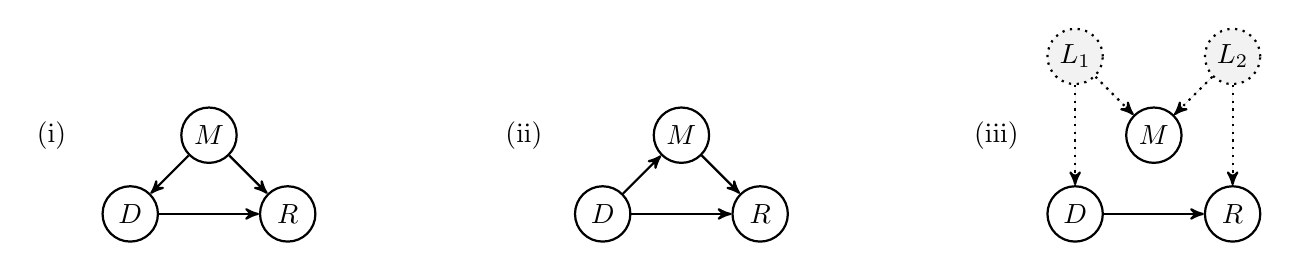
\begin{tikzpicture}
      \begin{scope}
        \node[var] (M) at (0,1) {$M$};
        \node[var] (D) at (-1,0) {$D$};
        \node[var] (R) at (1,0) {$R$};
        \draw[arr] (M)--(D);
        \draw[arr] (M)--(R);
        \draw[arr] (D)--(R);
        \node at (-2,1) {(i)};
      \end{scope}
      \begin{scope}[xshift=6cm]
        \node[var] (M) at (0,1) {$M$};
        \node[var] (D) at (-1,0) {$D$};
        \node[var] (R) at (1,0) {$R$};
        \draw[arr] (D)--(M);
        \draw[arr] (M)--(R);
        \draw[arr] (D)--(R);
        \node at (-2,1) {(ii)};
      \end{scope}
      \begin{scope}[xshift=12cm]
        \node[var] (M) at (0,1) {$M$};
        \node[var] (D) at (-1,0) {$D$};
        \node[var] (R) at (1,0) {$R$};
        \node[varh] (L1) at (-1,2) {$L_1$};
        \node[varh] (L2) at (1,2) {$L_2$};
        \draw[arr] (D)--(R);
        \draw[arrh] (L1)--(M);
        \draw[arrh] (L2)--(R);
        \draw[arrh] (L1)--(D);
        \draw[arrh] (L2)--(M);
        \node at (-2,1) {(iii)};
      \end{scope}
    \end{tikzpicture}
  }
\caption{Different hypothetical causal graphs, where $R$ stands for \emph{Recovery}, $D$ for taking the \emph{Drug}, and $M$ has different interpretations in cases (i), (ii) and (iii).\label{fig:Simpson}}
\end{figure}

Suppose you believe that an SCM with causal graph as in Figure \ref{fig:Simpson}(i) applies, where $M$ denotes gender of the patient (male/female).

\begin{enumerate}[label=\alph*)]
  \item \label{Simpson_1} \question{Apply the back-door criterion to obtain a formula that expresses $p(r \given \intervene(D=d))$ in terms of observable
quantities (i.e., in terms of marginal or conditional distributions where the \emph{do}-operator does not appear).
%In this case, we need to adjust for $\{M\}$ when calculating $p(R \given \intervene(D))$:
%      $$p(R \given \intervene(D)) = \sum_{M} p(R \given D, M) p(M) \ne p(R \given D)$$
}
\answer{We are looking for a subset of covariates that satisfies the assumptions of the back-door criterion. There are only two possible
subsets of covariates in this simple case: $\emptyset$ and $\{M\}$. According to the back-door criterion, we can adjust for $\{M\}$:
$$p(R \given \intervene(D)) = \sum_{M} p(R \given D, M) p(M).$$}

\item \question{Is $p(r \given \intervene(D=d)) = p(r \given d)$ in this case?}
\answer{No, for this causal model $p(R \given \intervene(D)) \ne p(R \given D)$ (except possibly for specifically tuned parameters of the model). Indeed,
note that $p(R \given D) = \sum_{M} p(R \given D, M) p(M \given D)$, and for the model in Figure \ref{fig:Simpson}(i), in general $p(M) \ne p(M \given D)$ (because of Bayes' theorem).}

\item \question{What would be your advice for a patient with unknown gender?}
\answer{First of all, one should realize that treating the patient is an \emph{intervention}: we are actively setting the random variable $D$ to some value.
Therefore, we are interested in the quantity $p(R \given \intervene(D))$, and not in $p(R \given D)$ (which lead to the paradox). We can calculate
    $p(R \given \intervene(D))$ using the adjustment formula in \ref{Simpson_1}. As $p(R|D=1,M) < p(R|D=0,M)$ for both genders, the same will hold for a mixture:
$p(R \given \intervene(D=1)) < p(R \given \intervene(D=0))$. So assuming
the causal structure in Figure \ref{fig:Simpson}(i), the advice would be not to take the drug.}
\end{enumerate}

Now suppose that instead, you believe that an SCM with causal graph as in Figure \ref{fig:Simpson}(ii) applies. Intuitively, this would be quite unlikely, as we
know that most drugs don't change gender, but we could have used a slightly different story where the variable $M$ has a different interpretation
(for example, ``blood pressure''), and then this causal structure would also be a plausible one.

\begin{enumerate}[resume*]
  \item \question{Again, use the back-door criterion to express $p(r \given \intervene(D=d))$ in terms of observable quantities.}
\answer{Now $M$ is a descendant of $D$, so we cannot use $\{M\}$ for adjustment. There are no back-door paths $D \leftarrow \dots \dots R$, so
$\emptyset$ is sufficient for adjustment:
$$p(R \given \intervene(D)) = p(R \given D)$$}

\item \question{Is $p(r \given \intervene(D=d)) = p(r \given d)$ in this case?}
\answer{Yes.}

\item \label{Simpson_2} \question{What would be your advice for a patient with unknown $M$ (say, blood pressure) in this case?}
\answer{As $p(R \given D=1) > p(R \given D=0)$, this means that now $p(R \given \intervene(D=1)) > p(R \given \intervene(D=0))$. So assuming the causal
structure is as in Figure \ref{fig:Simpson}(ii), the advice for (all) patients is to take the drug.}
\end{enumerate}

Finally, suppose that you believe that the SCM has the causal graph of Figure \ref{fig:Simpson}(iii).

\begin{enumerate}[resume*]
  \item \question{Invent an interpretation of $M$ and the two latent variables $L_1,L_2$ yourself that could match the causal model depicted in Figure \ref{fig:Simpson}(iii).}
\answer{Left to the imagination of the reader.}

\item \question{Express $p(r \given \intervene(D=d))$ in terms of \emph{observable} quantities.}
\answer{$\emptyset$ is sufficient for adjustment according to the back-door criterion, so
$$p(R \given \intervene(D)) = p(R \given D).$$}

\item \question{Is $p(r \given \intervene(D=d)) = p(r \given d)$ in this case?}
\answer{Yes.}

\item \question{Again, what would be your advice for a patient with unknown $M$ in this case?}
\answer{Same as in \ref{Simpson_2}: all patients should take the drug.}
\end{enumerate}

Conclusion: whether or not you should prescribe the drug depends on which causal model you believe to apply to this situation. 
The fact that different causal models will lead to different conclusions should not be paradoxical, it is another illustration that
``correlation does not imply causation''.

\subsection{Y-structure}

\begin{theorem}[Global Markov Property]
  For an acyclic SCM, the following \emph{Global Markov Property} holds:
  $$\B{X} \dsep_{\C{G}(\C{M})} \B{Y} \given \B{Z} \qquad \implies \qquad \B{X} \indep_{p_{\C{M}}} \B{Y} \given \B{Z}$$
  for all subsets $\B{X}, \B{Y}, \B{Z}$ of nodes.
\end{theorem}

Given an SCM $\C{M}$ with the following causal graph:
\begin{center}
  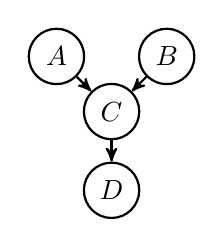
\begin{tikzpicture}
    \node[var] (A) at (-0.7,0.7) {$A$};
    \node[var] (B) at (0.7,0.7) {$B$};
    \node[var] (C) at (0,0) {$C$};
    \node[var] (D) at (0,-1) {$D$};
    \draw[arr] (A)--(C);
    \draw[arr] (B)--(C);
    \draw[arr] (C)--(D);
  \end{tikzpicture}
\end{center}

\question{Which (conditional) independences in $p_{\C{M}}$ are implied by the Global Markov Property?}

\subsection{LCD}

\begin{theorem}[Cooper, 1997]
Given an acyclic SCM $\C{M}$ with three endogenous variables $C,X,Y$. If:
\begin{compactenum}
  \item $X \to C \notin \C{G}(\C{M})$, 
  \item $Y \to C \notin \C{G}(\C{M})$,
  \item $C \notindep_{p_{\C{M}}} X$, 
  \item $X \notindep_{p_{\C{M}}} Y$,
  \item $C \indep_{p_{\C{M}}} Y \given X$, 
  \item Faithfulness holds, i.e., the Global Markov Property gives \emph{all} (conditional) independences in $p_{\C{M}}$.
\end{compactenum}
  Then $X \to Y \in \C{G}(\C{M})$, $C \to Y \notin \C{G}(\C{M})$, $X \leftrightarrow Y \notin \C{G}(\C{M})$, $C \oto Y \notin \C{G}(\C{M})$.
\end{theorem}

\question{Prove this theorem by considering for each possible ADMG $\C{G}(\C{M})$ whether it satisfies the assumptions.\\
(Hint: could there be an edge between $C$ and $Y$?)}
\answer{
\begin{center}
  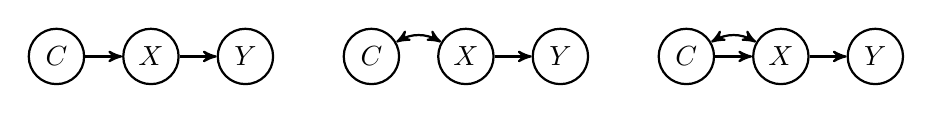
\begin{tikzpicture}
      \begin{scope}
        \node[var] (X) at (-1.2,0) {$C$};
        \node[var] (Y) at (0,0) {$X$};
        \node[var] (Z) at (1.2,0) {$Y$};
        \draw[arr] (X) edge (Y);
        \draw[arr] (Y) edge (Z);
      \end{scope}
      \begin{scope}[xshift=4cm]
        \node[var] (X) at (-1.2,0) {$C$};
        \node[var] (Y) at (0,0) {$X$};
        \node[var] (Z) at (1.2,0) {$Y$};
        \draw[biarr, bend left] (X) edge (Y);
        \draw[arr] (Y) edge (Z);
      \end{scope}
      \begin{scope}[xshift=8cm]
        \node[var] (X) at (-1.2,0) {$C$};
        \node[var] (Y) at (0,0) {$X$};
        \node[var] (Z) at (1.2,0) {$Y$};
        \draw[arr] (X) edge (Y);
        \draw[biarr, bend left] (X) edge (Y);
        \draw[arr] (Y) edge (Z);
      \end{scope}
  \end{tikzpicture}\end{center}}

%\bibliographystyle{apalike}
%\bibliography{simpsons-paradox}

\end{document}
